%!TEX root = dissertacao.tex
\section{DIFERENÇA ENTRE TEMPLATES}
\label{sec:resultadosParciais}
Neste capítulo apresenta-se o desenvolvimento da operação de diferença entre templates com $k=2$, introduz-se a operação de geração de templates de exceção, e demonstra-se uma série de passos que, utilizando templates, pode auxiliar na busca de ACs de raio 3 que tem a possibilidade de solucionar o problema de paridade.

\subsection{Templates de Exceção}
Alguns templates apresentam em seus campos valores que, quando expandidos, gerarão substituições inválidas e, por consequência, regras inválidas. O template $T_o = (x_7, x_6, x_5, 1 - x_1 - x_5, 2 - x_1 - x_2, x_2, x_1, 0)$ com $k=2$ é um exemplo disso. É trivial perceber que qualquer expansão do template $T_o$ que tenha o conjunto de substituições $\{x_1 = 1, x_5 = 1\}$ fará com que a posição 4 do template apresente o valor $2$, que não pertence ao intervalo $[0,k-1]$; da mesma maneira, qualquer expansão do template $T_o$ que tenha o conjunto de substituições $\{x_1 = 0, x_2 = 0\}$ fará com que a posição 3 do template também apresente um valor que não pertence ao intervalo $[0,k-1]$. Um \textit{template de exceção} é um template que apresenta esses conjuntos substituições que levam um template passado com parâmetro a apresentar substituições fora do intervalo inteiro $[0, k-1]$. Já o conjunto de \textit{template de exceção} de um template representa todos os templates de exceção encontrados apartir do template passado como parâmetro. O conjunto de templates de exceção do template $T_o$, utilizado como exemplo, pode ser representado pela Eq. \ref{eq:exceptionsTemplates}.

\begin{equation}
C_e = \{(x_7, x_6, 1, x_4, x_3, 1, x_2, x_0),(x_7, x_6, x_5, x_4, x_3, 0, 0, x_0)\}
\label{eq:exceptionsTemplates}
\end{equation}

Formalmente, a operação geradora de templates de exceção $X$ gera um conjunto $C_e$ com todos os templates de exceção do template $T_o$ passado como parâmetro. A operação que gera o conjunto templates de exceção de um template pode ser descrita em mais detalhes da seguinte maneira:
\begin{equation}
\begin{split}
X(T_o)= C_e \\
C_e = \{T_1,T_2,\dots, T_n\}\\
\end{split}
\end{equation}

O algoritmo dessa operação primeiro encontra todas as posições que não apresentem apenas variáveis livres ou constantes. O algoritmo gera então para cada uma das posições encontradas todas as substituições possíveis, dentro do intervalo $[0,k-1]$, para cada uma das variáveis presentes na posição. Por fim, verifica se a solução com as substituições possíveis levam valores fora dos intervalos $[0,k-1]$.

Para exemplificar, considere o template $T_{o} = (1, x_6, x_5, 1 - x_1 - x_2, 2 - x_1 - x_2, x_2, x_1, 0)$. O primeiro passo do algoritmo é encontrar um conjunto com as posições que não apresentem apenas constantes ou variáveis livres, obtendo-se assim $\{\{1 - x_1 - x_2\}, \{2 - x_1 - x_2\}\}$. Então, aplica-se à cada um dos itens do conjunto obtido todas as combinações possíveis das substituições de $x_1$ e $x_2$, conforme mostrado na Tabela \ref{tab:exceptionProcessA} e \ref{tab:exceptionProcessB} para $\{\{1 - x_1 - x_2\}, \{2 - x_1 - x_2\}\}$, respectivamente.
\begin{table}[h!]
\centering
\caption{Expansão do campo 1 - x_1 - x_2.}
	\begin{tabular}{ccc}
    \toprule
	$x_2$ & $x_1$ & Expansão do campo \\
    \midrule
	0	&	0	&	1 - x_1 - x_2 = 1	\\
	0	&	1	&	1 - x_1 - x_2 = 0	\\
	1	&	0	&	1 - x_1 - x_2 = 0	\\
	1	&	1	&	1 - x_1 - x_2 = -1	\\
    \bottomrule
	\end{tabular}
\label{tab:exceptionProcessA}
\end{table} 

\begin{table}[h!]
\centering
\caption{Expansão do campo 2 - x_1 - x_2.}
	\begin{tabular}{ccc}
    \toprule
	$x_2$ & $x_1$ & Expansão do campo \\
    \midrule
	0	&	0	&	2 - x_1 - x_2 = 2	\\
	0	&	1	&	2 - x_1 - x_2 = 1	\\
	1	&	0	&	2 - x_1 - x_2 = 1	\\
	1	&	1	&	2 - x_1 - x_2 = 0	\\
    \bottomrule
	\end{tabular}
\label{tab:exceptionProcessB}
\end{table}

Para finalizar a operação, o algoritmo seleciona as substituições que geram valores inválidos, e aplicam ela ao template base, gerando assim o conjunto de templates $C_e$, mostrado na  Eq. \ref{eq:exceptionsTemplates2}.

\begin{equation}
C_e = \{(x_7, x_6, x_5, x_4, x_3, 1, 1, x_0),(x_7, x_6, x_5, x_4, x_3, 0, 0, x_0)\}
\label{eq:exceptionsTemplates2}
\end{equation}

A operação que gera os templates de exceção foi apresentada por Soares, Verardo e
de Oliveira (\citeyear{soares2016difference}) e é importante por ser essencial para a operação de diferença entre templates. 

É importante frisar que essa é uma operação com complexidade $O(c^n)$, onde $n$ é o número de variáveis nas posições que não apresentem apenas variáveis livres ou constantes. Por conta disso, a operação de diferença pode se mostrar demasiadamente custosa quando aplicadas a templates com muitas dependências entre variáveis, tais como os templates de conservabilidade e conservabilidade de paridade.

\subsection{Diferença entre Templates binários}
A operação de diferença entre templates binários $D_i$ é responsável por obter um conjunto $C_{di}$ com $n$ templates, os quais, quando expandidos (via a operação de expansão $E$), apresentam apenas as regras geradas pela expansão do template $T_m$ que não estejam também presentes na expansão do template de intersecção entre $T_s$ e $T_m$, chamado aqui de $T_i$. A operação de diferença pode ser descrita em mais detalhes da seguinte maneira:
\begin{equation}
\begin{split}
D_i(T_m,T_s)= C_{di} \Leftrightarrow E(C_{di}) = E(T_m) \setminus E(T_i) \\
T_i = I(T_m,T_s)\\
C_{di} = \{T_1,T_2,\dots, T_n\}\\
\end{split}
\end{equation}

A Figura \ref{fig:complement} ilustra essa operação, onde os templates $T_m$ e $T_s$ passados como parâmetro para a operação de diferença estão representado pelos dois círculos, e o conjunto $C_{di}$ retornado pela função está representado pela área em cinza na imagem.
\begin{figure}[h!]
  \centering
  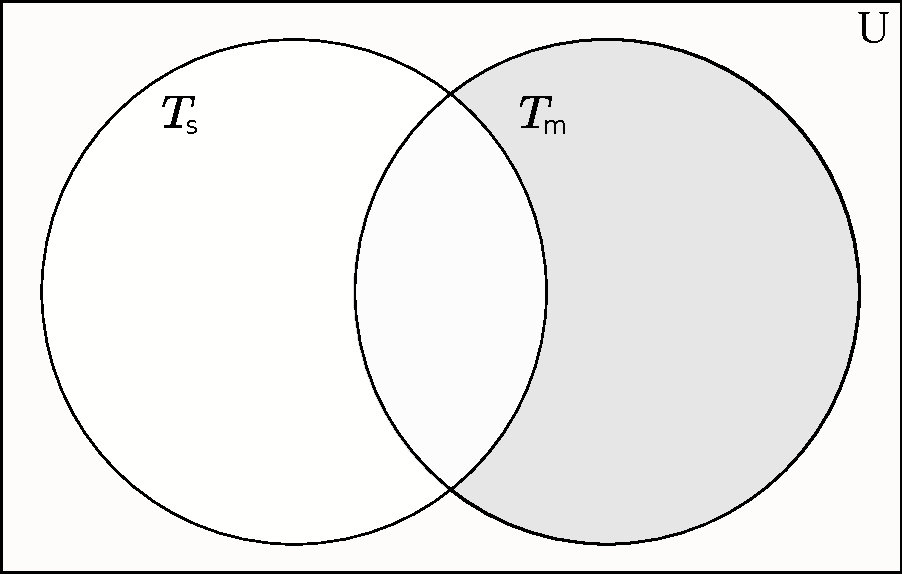
\includegraphics[width=.4\textwidth]{fig_complement2.pdf}
  \caption{Os círculos $T_m$ e $T_s$ são os templates que representam dois conjuntos de regras. Em cinza, $C_{di}$ é o conjunto de templates que representam o conjunto de regras retornado pela operação de diferença entre $T_m$ e $T_s$.}
  \label{fig:complement}
\end{figure}    

O processo que o algoritmo usa para encontrar a diferença entre dois templates é efetuado através de uma sequência de etapas. A primeira etapa consiste em encontrar o template $T_i$, que é a intersecção entre os templates $T_m$ e $T_s$, ambos recebidos como parâmetro. Em seguida, igualam-se os templates $T_m$ e $T_i$, obtendo-se assim combinações lógicas de equações. Após remover eventuais equações tautológicas, o algoritmo aplica a operação de negação nas equações e troca o operador lógico $\wedge$ por $\vee$, que, no caso binário, consistem apenas em efetuar as permutações $\rho = (0 \rightarrow 1, 1 \rightarrow 0, \wedge \rightarrow \vee)$ ao resultado final das equações. Esse sistema é então solucionado, resultando num conjunto com diversos conjuntos de regras de substituições, as quais são aplicadas ao template $T_i$, gerando um conjunto de templates que é parte do resultado dessa operação. Um segundo conjunto de templates será a outra parte do resultado. Esse conjunto será gerado a partir da intersecção de cada um dos templates de exceção do template $T_i$ com o template $T_m$.

Para melhor visualizar essas etapas, considerem-se os templates $T_m = (x_7, x_6, x_5, x_4, x_3,\\ x_1, x_1, x_0)$ e $T_s = (x_7, x_6, x_3 + x_1, 1 - x_1, x_3, x_1, x_1, 0)$, ambos com $k=2$ e $r=1$. Esses templates serão primeiramente passados para a operação de intersecção, gerando assim o template $T_i = (x_7, x_6, x_3 + x_1, 1 - x_1, x_3, x_1, x_1, 0)$. Na sequência, igualam-se os templates $T_m$ e $T_i$, o que gera o sistema de equações mostrado na Eq. \eqref{eq:complement}.
\begin{equation}
\left\{\begin{matrix}
x_7 & = & x_7	\\ 
x_6 & = & x_6	\\ 
x_5 & = & x_3 + x_1	\\ 
x_4 & = & 1 - x_1 \\ 
x_3 & = & x_3	\\ 
x_1 & = & x_1	\\ 
x_1 & = & x_1	\\ 
x_0 & = & 0
\end{matrix}\right.
\label{eq:complement}
\end{equation}

Esse sistema deve ser representado através de combinações lógicas de equações, como se pode ver na Eq. \eqref{eq:logicalComplement}, que é equivalente à Eq. \eqref{eq:complement}.
\begin{equation}
\begin{split}
x_7 = x_7	\wedge  
x_6 = x_6	\wedge  
x_5 = x_3 + x_1	\wedge  
x_4 =   1 - x_1 \wedge  \\
x_3 = x_3	\wedge  
x_1 = x_1	\wedge  
x_1 = x_1	\wedge  
x_0 = 0
\end{split}
\label{eq:logicalComplement}
\end{equation}

Antes de solucionar a Eq. \eqref{eq:logicalComplement}, o algoritmo elimina todas as equações tautológicas e troca todo operador lógico $\wedge$ por $\vee$; como resultado, obtêm-se a Eq. \eqref{eq:logicalComplement1}.
\begin{equation}
x_5 = x_3 + x_1 \vee x_4 = 1 - x_1 \vee x_0 = 0
\label{eq:logicalComplement1}
\end{equation}

Por fim,  aplica-se a operação de negação nas equações. No caso binário basta efetuar a permutação $\rho$, que também pode ser feita por meio da função $f(x) = 1 - x$. A Eq. \eqref{eq:logicalComplement2} representa a combinação lógica de equações que resulta das operações precedentes.
\begin{equation}
x_5 = 1 - (x_3 + x_1) \vee x_4 = 1 - (1 - x_1) \vee x_0 = 1 - 0
\label{eq:logicalComplement2}
\end{equation}

A etapa de troca do operador lógico e de permutação $\rho$ são a base desta operação, pois essas etapas determinam que se qualquer campo de um template resultar numa regra com um valor diferente do esperado no template original, esse campo deve ser considerado para a criação dos templates de diferença.

Continuando, a combinação lógica de equações da Eq. \eqref{eq:logicalComplement2} é então solucionada, resultando no conjunto solução $S = \{\{x_0 \to 1\}, \{x_4 \to x_1\}, \{x_5 \to 1 - x_1 - x_3\}\}$. Perceba-se que $S$ apresenta mais de um conjunto de substituições e, portanto, cada um deles deve ser utilizado para realizar as substituições no template $T_m$. Essas substituições fazem com que se obtenha o conjunto de templates $C_{d1}$, representados pela Eq. \eqref{eq:logicalComplement3}. 
\begin{equation}
\begin{split}
C_{d1} = \{\\(x_7, x_6, x_5, x_4, x_3, x_1, x_1, 1), \\(x_7, x_6, x_5, x_1, x_3, x_1, x_1, x_0), \\(x_7, x_6, 1 - x_1 - x_3, x_4, x_3, x_1, x_1, x_0)\\\}
\end{split}
\label{eq:logicalComplement3}
\end{equation}

Os templates do conjunto $C_{d1}$ farão parte do conjunto $C_{di}$ resultante da operação de diferença. Entretanto, é necessário verificar se o template $T_i$ possui combinações de substituições que o levem a gerar regras inválidas. Isso é feito passando o template $T_i$ para a operação geradora de template de exceção, o que resulta no conjunto de templates $\{(x_7, x_6, x_5, x_4, 1, x_2, 1, x_0)\}$ (que, no caso, só possui 1 elemento). Os templates desse conjunto são então interseccionados com o template $T_m$, resultando no conjunto $C_e = \{(x_7, x_6, x_5, x_4, 1, 1, 1, x_0)\}$. Por fim, faz-se a unificação dos conjuntos $C_{d1}$ e $C_e$, obtendo-se o conjunto de templates $C_{di}$, representado pela Eq. \ref{eq:complementionSet}.
\begin{equation}
\begin{split}
C_{d1} = \{\\(x_7, x_6, x_5, x_4, x_3, x_1, x_1, 1), \\(x_7, x_6, x_5, x_1, x_3, x_1, x_1, x_0), \\(x_7, x_6, 1 - x_1 - x_3, x_4, x_3, x_1, x_1, x_0), \\(x_7, x_6, x_5, x_4, 1, 1, 1, x_0)\\\}
\label{eq:complementionSet}
\end{split}
\end{equation}

A operação de diferença $D_i$ também pode ser realizada sem se efetuar a intersecção. Nesse caso, a operação sem intersecção, chamada aqui apenas por $D$, encontrará um conjunto de templates $C_d$. A expansão dos templates de $C_{d}$ apresentará apenas as regras geradas pela expansão do template $T_m$ que não estejam também presentes na expansão do template $T_s$. Essa operação pode ser descrita em mais detalhes da seguinte maneira:
\begin{equation}
\begin{split}
D(T_m,T_s)= C_d \Leftrightarrow E(C_d) = E(T_m) \setminus E(T_s) \\
C_d = \{T_1,T_2,\dots, T_n\}\\
\end{split}
\end{equation}

O processo que o algoritmo da operação $D$ usa para encontrar a diferença entre dois templates é bem parecido com o do algoritmo da operação $D_{i}$. Primeiramente, igualam-se os templates $T_m$ e $T_s$, obtendo-se assim combinações lógicas de equações. Após remover eventuais equações tautológicas, o algoritmo aplica a operação de negação nas equações e troca o operador lógico $\wedge$ por $\vee$. Esse sistema é então solucionado, resultando num conjunto com diversos conjuntos de regras de substituições. E após eliminar desse conjunto eventuais substituições envolvendo variáveis que não pertençam ao $T_m$, esses conjuntos de regras de substituição são aplicados ao template $T_m$, gerando o conjunto de templates que é parte do resultado dessa operação. Um segundo conjunto de templates, composto pela intersecção de cada um dos templates de exceção do template $T_s$ com o template $T_m$, será a outra parte do resultado.

Os algoritmos $D$ e $D_i$ apresentam como resultado os conjunto de templates $C_d$ e $C_{di}$, respectivamente. $C_d$ e $C_{di}$ podem ser diferentes mesmo quando $D$ e $D_i$ recebem os mesmos templates como entrada. Mas ambos contêm exatamente as mesmas regras quando se expande os templates dos conjuntos.

\section{DISCUSSÃO E TESTES}
\label{sec:discussoesETestes}
A implementação das operações de diferença foi desenvolvida na linguagem do software \textit{Wolfram Mathematica} \cite{woframMathematica10} e na mesma linguagem foram criados os testes unitários que verificam se o \textit{output} da operação está correto de acordo com os possíveis \textit{input} dados a ela. Todos os testes receberam dois templates, $T_m$ e $T_s$, expandiram esses dois templates individualmente, e depois subtraíram das regras encontradas na expansão de $T_m$ todas as regras representadas por $T_s$. O resultado da diferença entre $T_m$ e $T_s$ é o conjunto de regras $C_{exp}$. Esse conjunto de regras $C_{exp}$ deve ser idêntico às regras geradas pela expansão dos templates resultantes da operação de diferença entre os templates $T_m$ e $T_s$. Por conta desta custosa forma de teste, os testes dessa operação se concentraram nos raios 1, 2 e 3.

Uma importante questão sobre a expansão do conjunto de regras $C_{exp}$, encontrado pela operação de diferença, é definir qual será o pós-processamento da operação de expansão que deve ser usado com esses templates. A operação de pós-processamento a ser utilizada na operação de diferença sempre será a mesma utilizada no template $T_m$ passado como parâmetro, acrescida da operação de filtro das regras inválidas caso essa operação já não tenha sido feita. Isto porque a operação de diferença deve representar todas as regras válidas da expansão de $T_m$ que não sejam representadas por $T_s$. Assim, caso $T_m$ e $T_s$ não tenham intersecção, o resultado deve ser apenas o template $T_m$ com o mesmo pós-processamento.

Nos testes para todos os raios foi gerado um conjunto de templates e, a partir dele, geraram-se todos os pares de combinações possíveis. Por fim, foi realizado o teste da operação de diferença com cada um dos pares de template gerados.

Para os testes com $r = 1$, cada um dos templates do conjunto usado para os testes representava uma das seguintes propriedades estáticas: conservabilidade de estados; confinamento; totalidade; semi-totalidade; e invariância  à troca de cor. Além desses templates, também foi utilizado o template base, que representa todas as regras do espaço.

Para os testes com $r = 2$, os templates usados representavam as seguintes propriedades estáticas: Conservabilidade de estados; totalidade; semi-totalidade; e invariância à troca de cor. Já para os testes $r = 3$, os templates de teste representavam apenas as propriedades estáticas de totalidade e semi-totalidade. Foram feitos testes com menos propriedades de acordo com o raio pois esses testes envolvem expansões, que para algumas dessas propriedades consiste em enumerar um número muito grande de regras. Assim os testes foram feitos apenas com propriedades em que a expansão dos templates encontrados consista em enumerar menos que $2^{16}$ regras. A Tabela \ref{tab:differenceTests} mostra em mais detalhes os templates de quais propriedades estáticas foram utilizados para os testes da operação de diferença e em quais tamanhos de raio.

\begin{table}[h!]
\centering
\caption{Propriedades estáticas utilizadas para o teste da operação de diferença em cada raio}
\resizebox{\textwidth}{!}{%
\begin{tabular}{l|lllll|}
\cline{2-6}
& \multicolumn{5}{c|}{Template minuendo ($T_m$)} \\ \cline{1-1}
\multicolumn{1}{|l|}{Template subtraendo ($T_s$)}                  
& totalidade
& semi-totalidade
& \begin{tabular}[c]{@{}l@{}}conservabilidade\\ de estados\end{tabular} 
& \begin{tabular}[c]{@{}l@{}}invariância à\\ troca de cor\end{tabular}  
& confinamento 
\\ \cline{2-6} 

\multicolumn{1}{|l|}{totalidade} 				  & Raio 1, 2 e 3& Raio 1, 2 e 3  & Raio 1 e 2& Raio 1 e 2& Raio 1	\\
\multicolumn{1}{|l|}{semi-totalidade} 			  & Raio 1, 2 e 3& Raio 1, 2 e 3  & Raio 1 e 2& Raio 1 e 2& Raio 1	\\
\multicolumn{1}{|l|}{conservabilidade de estados} & Raio 1 e 2	 & Raio 1 e 2	  & Raio 1 e 2& Raio 1 e 2& Raio 1	\\
\multicolumn{1}{|l|}{invariância  à troca de cor} & Raio 1 e 2	 & Raio 1 e 2	  & Raio 1 e 2& Raio 1 e 2& Raio 1	\\
\multicolumn{1}{|l|}{confinamento}                & Raio 1		 & Raio 1		  & Raio 1	& Raio 1	& Raio 1	\\ \hline
\bottomrule
\end{tabular}%
}
\label{tab:differenceTests}
\end{table}

Ademais, esses testes mostraram que a operação de diferença está funcionando para diversos templates, sem a necessidade de operações específicas para cada um dos templates.

É importante explicitar que a implementação do algoritmo que executa a operação de diferença entre templates ainda não permite trabalhar com $k\neq 2$, pois a negação das equações são feitas por meio da função $f(x) = 1 - x$.

\subsection{Templates aplicados no problema de paridade}
O desenvolvimento da operação de diferença entre template permite diversas possibilidades de aplicação.
Uma das possibilidades é no problema de paridade. 
Ainda não se sabe se existem regras de raio 3 que solucionem o problema de paridade \cite{Betel2013}. 
Mas o uso de templates e suas operações podem ser uma forma interessante de restringir o conjunto de regras na busca dessa solução.

As regras dos ACs que solucionam o problema de paridade têm algumas propriedades estáticas que podem ser trivialmente percebidas. 
Um AC que resolva o problema de paridade sempre será confinado, tendo em vista que as vizinhanças homogêneas não devem levar a transições de estado ativas, a qual é a única restrição de variável nos templates confinados para ACs binários. 
O espaço das regras confinadas de raio 3 ainda é muito grande; entretanto, essa não é a única propriedade estática que um AC que resolva o problema de paridade apresenta.  Nesse sentido, também é necessário que ele não seja conservativo, visto que, se a soma dos estados do AC não mudar, ele nunca convergirá como propõe o problema. 
Por fim, espera-se que um AC que resolva o problema de paridade seja conservativo de paridade.

Dada a possibilidade de se obter os templates para todas essas propriedades, é também possível utilizar esses templates e as operações de diferença e intersecção para expressar esse espaço de busca para a solução do problema de paridade.
Para expressar esse espaço, basta efetuar a intersecção dos templates de confinamento com o template de conservabilidade de paridade, visto que ambas as propriedades são necessárias. Entretanto, vale frisar que essa intersecção gera o próprio template de paridade, não fazendo diferença para o resultado final.
Posteriormente, deve-se efetuar a operação de diferença com o template obtido pela primeira intersecção com o template das regras conservativas de estado, já que a conservabilidade de estado impede a resolução do problema de paridade.

Formalmente, essas operações de conjuntos entre os templates podem ser representadas através da Eq. \eqref{eq:operationsTemplateParidade}, sendo que $T_{confinado}$ representa o template das regras confinadas, $T_{conservaparidade}$ representa o templates das regras que conservam a paridade, e ${T}_{conservaestados}$ indica o template de regras conservativas. O resultado dessa operação é $T_{paridade}$, o qual representa um conjunto de templates que restringem um pouco mais as regras com possibilidades de solucionar o problema de paridade.
\begin{equation}
T_{paridade} = (T_{conservaparidade} \cap T_{confinado}) - {T}_{conservaestados}
\label{eq:operationsTemplateParidade}
\end{equation}

Entretanto, apesar de formalmente possível, a realização dessas operações não se mostrou produtiva. Isto ocorre pois a operação de exceção, utilizada pela operação de diferença, tem complexidade $O(c^n)$, onde $n$ é o número de variáveis nas posições que não apresentem apenas variáveis livres ou constantes nos templates. Deste modo, gerar os templates de exceção do template $T_{conservaestados}$ é tão custoso quanto expandir todas as regras desse template.

Dito isto, é mais simples utilizar o template $T_{conservaestados}$ com uma função de pós-processamento alternativa que elimine todas as tabelas $k$-árias que não apresentem campos inválidos, e aplique $mod$ $2$ nas restantes. Assim  esse mesmo template vai representar apenas as regras que mantenham a paridade mas não apresentem a propriedade de conservabilidade de estados. Também poderá ser aplicado nesse template operações de intersecção ou diferença com outros templates de modo a se restringir ainda mais o espaço de busca.